\documentclass{article}
\usepackage{graphicx}
\usepackage{amsmath}
\usepackage{rotating}
\setlength{\parskip}{1em}

\begin{document}

\title{Implementation of the Massey Sain algorithm}
\author{Carl Selig}

\maketitle
\newpage

\section{Inverting a discrete state-space model}
To implement Internal Model Control it is necessary to create both a model of the plant and an inverse of that model. The plant model is provided from [ANDY’S EWTEC PAPER] in the form of a state-space model. Creating a robust inverse of this model is a task for this project.

One potential approach is to convert the state-space system into a system of transfer functions. In this case the inverse is simply the reciprocal of the transfer function. This method is complicated by the fact that the plant is a 6x6 MIMO system. Generating corresponding transfer functions using inbuilt MATLAB methods results in 36 very high order transfer functions. Problems with this include:
\begin{itemize}
	\item{Over-fitting to the model}
	\item{Improper after being inverted, requiring a filter to be realisable}
	\item{Only practical to consider a maximum of 6 transfer functions, ignoring cross terms. (2 in practice)}
\end{itemize}


The Massey-Sain algorithm is an alternate method for creating a real-time inverse of a state space system. It was first presented in IEEE Transactions on Automatic Control, vol.14, 1969. Later it was summarised in a lecture given by Sundaram at the University of Illinois at Urbana-Champaign. The following derivation is paraphrased from Sundaram's lecture.

First it is necessary to convert the continuous time state-space model to a discrete time model. This is achieved using the ‘c2d’ function in MATLAB. Using discrete time also prevents any errors caused by the numerical methods of the Simulink solver.

First it is necessary to test whether or not the system is invertible. All discrete-time state space systems are of the form:
\begin{equation}
	x(t+1)=Ax(t)+Bu(t)
\end{equation}
\begin{equation}
	y(t)=Cx(t)+Du(t)
\end{equation}

Where x is the state vector; y is the output vector; u is the input vector; A is the state matrix; B is the input matrix; C is the output matrix; and D is the disturbance matrix.

For our system there is no disturbance input and so D is the zero matrix. It will not be shown in further equations.

Paraphrasing from Sundaram:
“A system has an inverse with delay $L$ if $u(t)$ can be uniquely determined from $y(t),y(t+1),…y(t+L)$  (and perhaps $x(t)$)”

So, we need to find the lowest possible value of L. It is possible to express later time-steps in terms of the current time step via substitution.
\[					%delimiters for 'displaymath' environment, no numbering.
	y(t+1)=Cx(t+1)
\]

Substituting equation 1:
\[
	y(t+1)= Ax(t)+Bu(t)
\]

This can be iterated for arbitrarily large timesteps. It can also be represented in a matrix format:

\[
	\begin{bmatrix}
		y(t)   \\
		y(t+1) \\
		y(t+2) \\
		\vdots \\
		y(t+L)
	\end{bmatrix}
	=
	\begin{bmatrix}
		C   \\
		CA  \\
		CA^2\\
		\vdots\\
		CA^L
	\end{bmatrix}
	x(t) +
	\left[
	\begin{array}{c|cccc}			%Have to use 'array' to do partitions
	0&0&0&\hdots&0						\\
	CB&0&0&\hdots&0						\\
	CAB&CB&0&\hdots&0					\\
	\vdots&\vdots&\vdots&\ddots&\vdots	\\
	CA^{L-1}B & CA^{L-2}B & CA^{L-3}B & \hdots & 0
	\end{array}
	\right]
	\left[
	\begin{array}{c}
		u(t)		\\
		\hline
		u(t+1)		\\
		u(t+2)		\\
		\vdots		\\
		u(t+L)
	\end{array}
	\right]
\]
\begin{equation}
=Y_{(t,L)} = O_Lx(t)+M_L U_{(t,L)}
\end{equation}

Where $O_L$ is analogous to the Observability of the system, and $M_L$ to its Measurability. The partitions show that $M_L$ contains the smaller matrix $M_{L-1}$. This can be iterated for all versions of $M_L$ down to $M_0$.

Massey \& Sain's theorem asserts that if the rank of $M_L$ minus the rank of $M_{L-1}$ is equal to the number of columns $'m'$ of $M_{L-1}$ then there exists a matrix $\mathcal{K}$ such that
\[
\mathcal{K}M_L =
\left[
\begin{array}{c|c}
I_m & 0
\end{array}
\right]
\]
Multiplying equation 3 by $\mathcal{K}$:
\[
\mathcal{K}Y_{t,L} = \mathcal{K}O_Lx(t) + u(t)
\]
Hence the input $u(t)$ can be expressed in terms of the outputs $Y_{t,L}$

\begin{equation}
u(t) = -\mathcal{K}O_Lx(t) + \mathcal{K}Y_{t,L}
\end{equation}

Similarly the state vector at time $t+1$ can be found by substituting equation 4 into equation 1
\begin{equation}
x(t+1) = (A-B\mathcal{K}O_L)x(t) + B\mathcal{K}Y_{t,L}
\end{equation}

Equations 4 and 5 together represent the inverse State-space model.

The task is now to see if there exists a value of L for our system that will satisfy the Massey-Sain theorem. In the case that there are multiple viable values of L the smallest value is preferable as any inverse constructed with it will have the smallest possible delay.

In the case of our 6 input, 6 output system
\begin{itemize}
\item{$M_0$ is the $6\times6$ zero matrix
\begin{flushright}
rank = 0, m = 6
\end{flushright}
}
\item{$M_1$ has the form
\[
\left[
\begin{array}{cc}
0	&	0	\\
CB	&	0	\\
\end{array}
\right]
\]
where $CB$ is a full-rank $6\times6$ matrix
\begin{flushright}
rank = 6
\end{flushright}
}
\end{itemize}

Therefore the system is invertible with $L=1$ since
\[
rank(M_1) - rank(M_0) = m_0
\]

As above the matrix $\mathcal{K}$ is formed by performing a pseudo-inverse of $M_1$ less the last 6 columns. This results in a $12\times6$ matrix. This is expected since
\[
Y_{t,L} = Y_{t,1} =
\begin{bmatrix}
y(t)	\\
y(t+1)
\end{bmatrix}
\]
so to find the inverse at the time-step $t+1$ the inverse system must be given both $y(t)$ and $y(t+1)$. since y is a $6\times1$ vector this makes $Y_{t,1}$ a $12\times1$ vector which matches the dimensions of $\mathcal{K}$.

The inverse is then constructed according to equations 4 and 5, and a one time-step delay is used to generate $y(t)$ at the timestep $t+1$.

This results in a robust inverse system. When used in the IMC loop it is able to perfectly track simple sinusoid input save for a delay of one time-step. It is hoped that this delay will be negligible for small time-steps.

\begin{sidewaysfigure}[h]
	\centering
	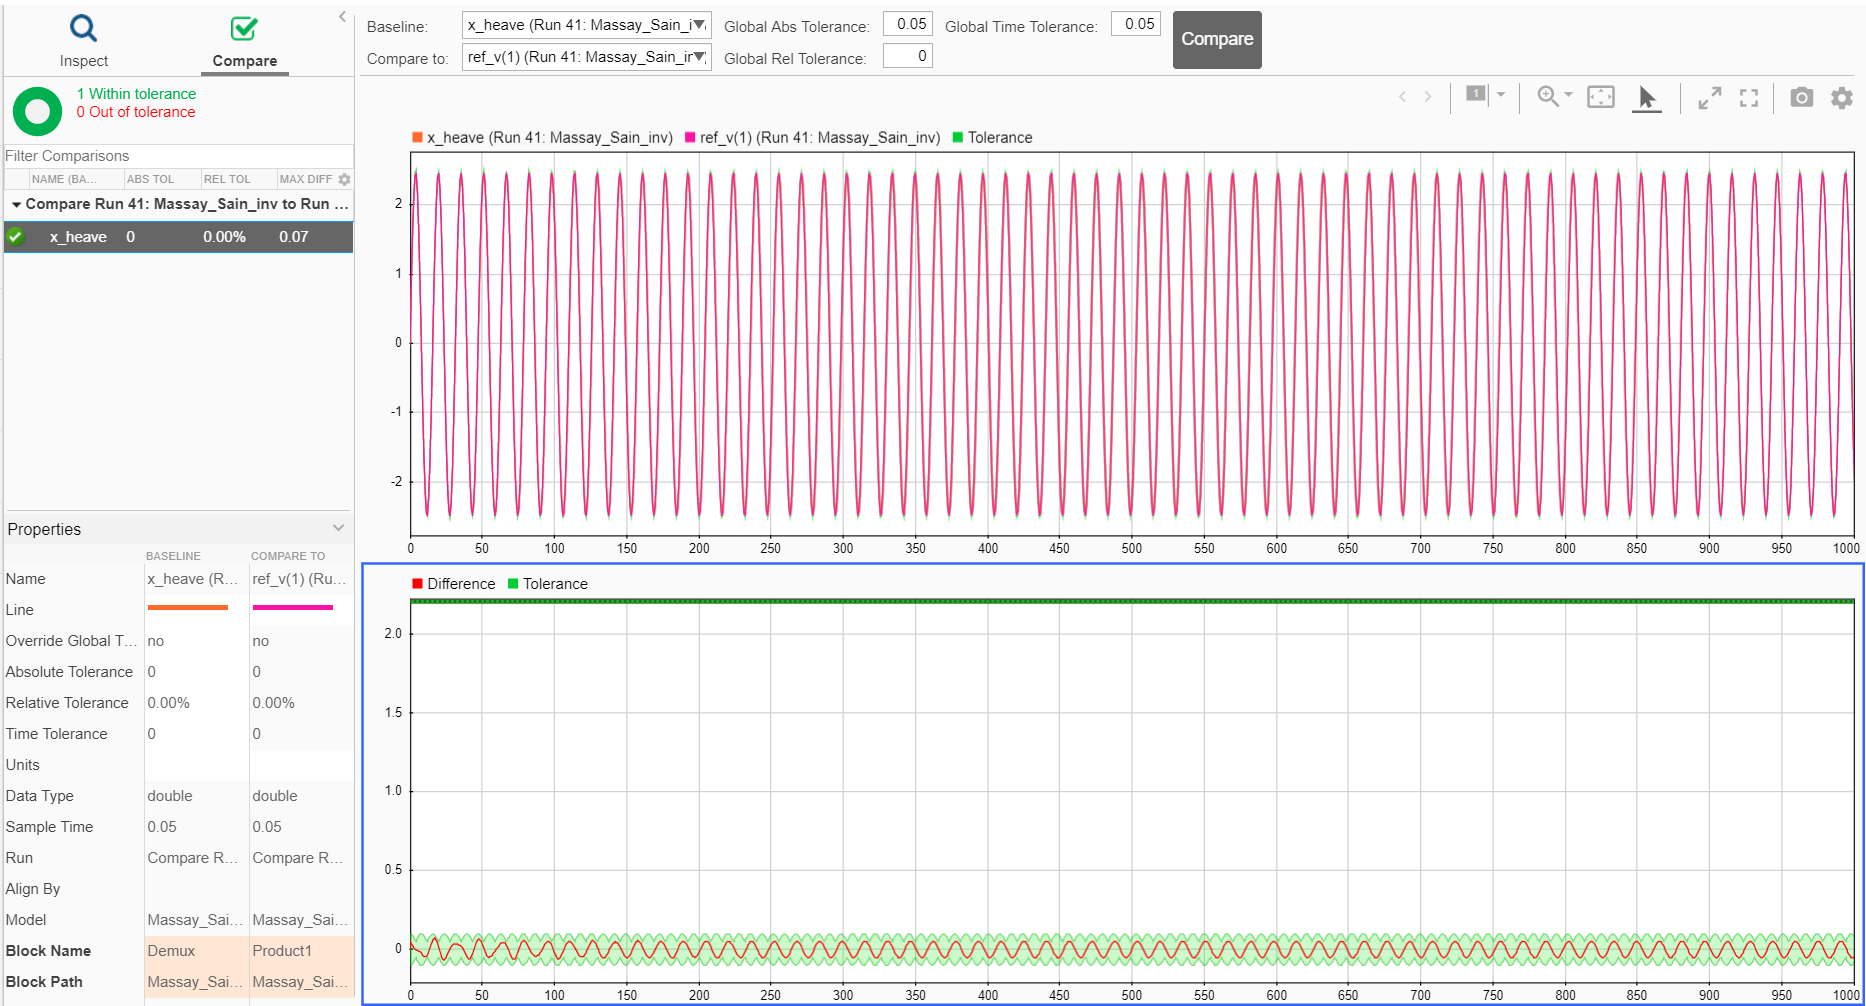
\includegraphics[scale=0.55]{heaveTracking}
	\caption{A simulink data inspector comparison of the heave input and the output of the control loop. The input was a sinusoid with amplitude $10^6m$ and frequency $0.4rads^{-1}$. The time step was $0.05s$. The output matches the input with a global tolerance of $0.05 units$.}
\end{sidewaysfigure}


\end{document}